\section{Inducing Emergent Abilities in Networks on Vision Tasks}
\label{sec:inducing_emergence_vision}

To demonstrate how emergent abilities can be induced by the researcher's choice of metric, we show how to produce emergent abilities in deep networks of various architectures: fully connected, convolutional, self-attentional.
We focus on vision tasks because abrupt transitions in vision models' capabilities have not been observed to the best of our knowledge; this is one reason why emergence in large language models is considered so interesting.
% Second, some vision tasks can be solved by modestly sized networks and therefore can enable us to construct entire model families with scales spanning multiple orders of magnitude.
% We specifically use simple networks on well-studied tasks to drive home the point that there is nothing new here.
For the convolutional example, see App. \ref{app:sec:inducing_emergence_vision}.

\paragraph{Emergent Reconstruction of CIFAR100 Natural Images by Nonlinear Autoencoders}

\begin{figure}
    \centering
    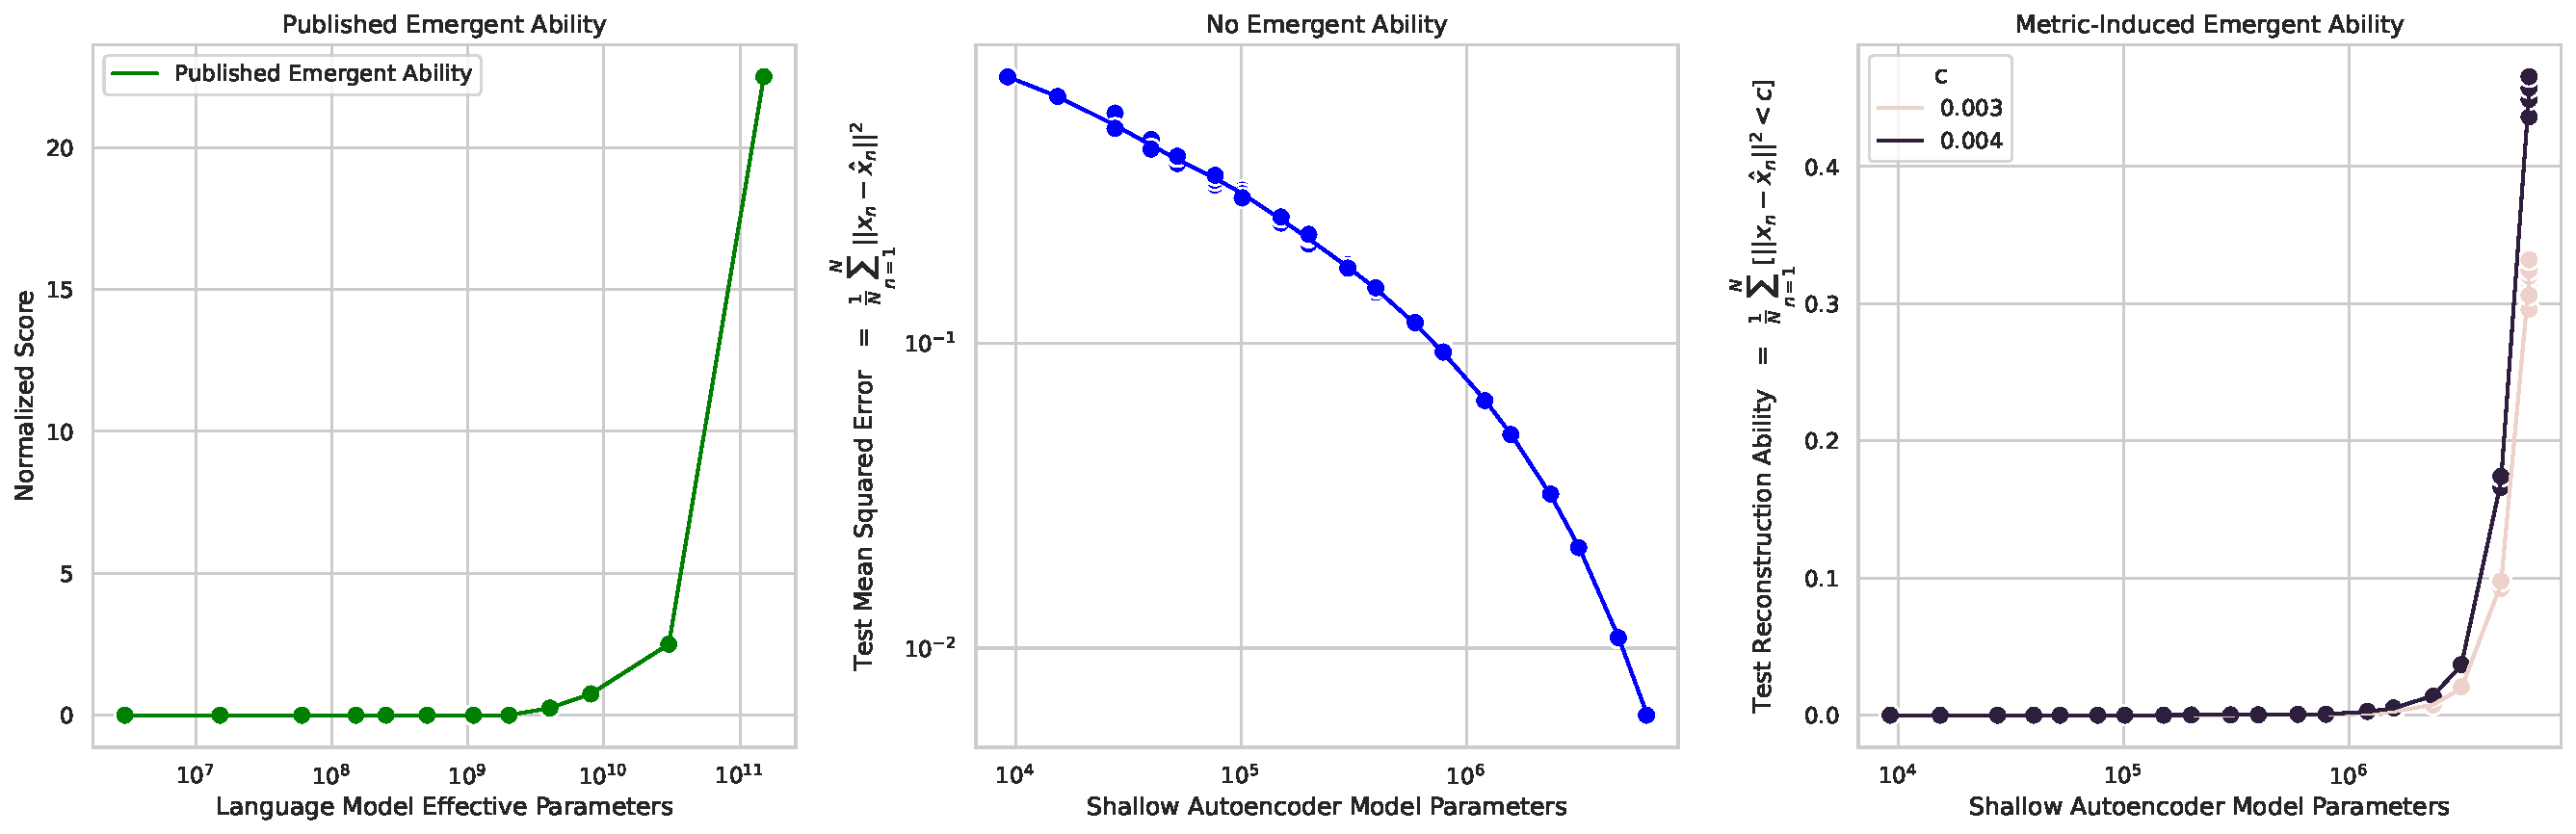
\includegraphics[width=0.9\textwidth]{figures/vision/no_emergence_and_emergence_dataset=cifar100.pdf}
    \caption{\textbf{Induced emergent reconstruction ability in shallow nonlinear autoencoders.} (A) A published emergent ability at the BIG-Bench Periodic Elements task \cite{srivastava2022beyond}. (B) Shallow nonlinear autoencoders trained on CIFAR100 \cite{krizhevsky09learningmultiple} display smoothly decreasing mean squared reconstruction error. (C) Using a newly defined Reconstruction$_c$ metric (Eqn. \ref{eq:reconstruction}) induces an unpredictable change.}
    \label{fig:vision_cifar100}
\end{figure}

We first induce an emergent ability to reconstruct images in shallow (i.e., single hidden layer) nonlinear autoencoders trained on CIFAR100 natural images \cite{krizhevsky09learningmultiple}.
To emphasize that the sharpness of the metric is responsible for emergent abilities, and to show that sharpness extends to metrics beyond Accuracy, we intentionally define a discontinuous metric that measures a network's ability to reconstruct a dataset as the average number of test data with squared reconstruction error below threshold $c$:
%
\begin{equation}
    \text{Reconstruction}_c \Big(\{x_n \}_{n=1}^N \Big) \; \defeq \;
    \frac{1}{N} \sum_n \mathbb{I} \Big[ ||x_n - \hat{x}_n||^2 < c \Big]
    \label{eq:reconstruction}
\end{equation}
where $\mathbb{I}(\cdot)$ denotes an indicator variable and $\hat{x}_n$ is the autoencoder's reconstruction of $x_n$.
The autoencoder family displays smoothly decreasing squared reconstruction error as the number of bottleneck units increases (Fig. \ref{fig:vision_cifar100}B). Under our newly defined Reconstruction$_c$ metric and for particular choices of $c$, the autoencoder family exhibits a sharp and seemingly unpredictable image reconstruction ability (Fig. \ref{fig:vision_cifar100}C) that qualitatively matches published emergent abilities (Fig. \ref{fig:vision_cifar100}A).
% , for the BIG-Bench Periodic Elements task 

\paragraph{Emergent Classification of Omniglot Characters by Autoregressive Transformers}

\begin{figure}
    \centering
    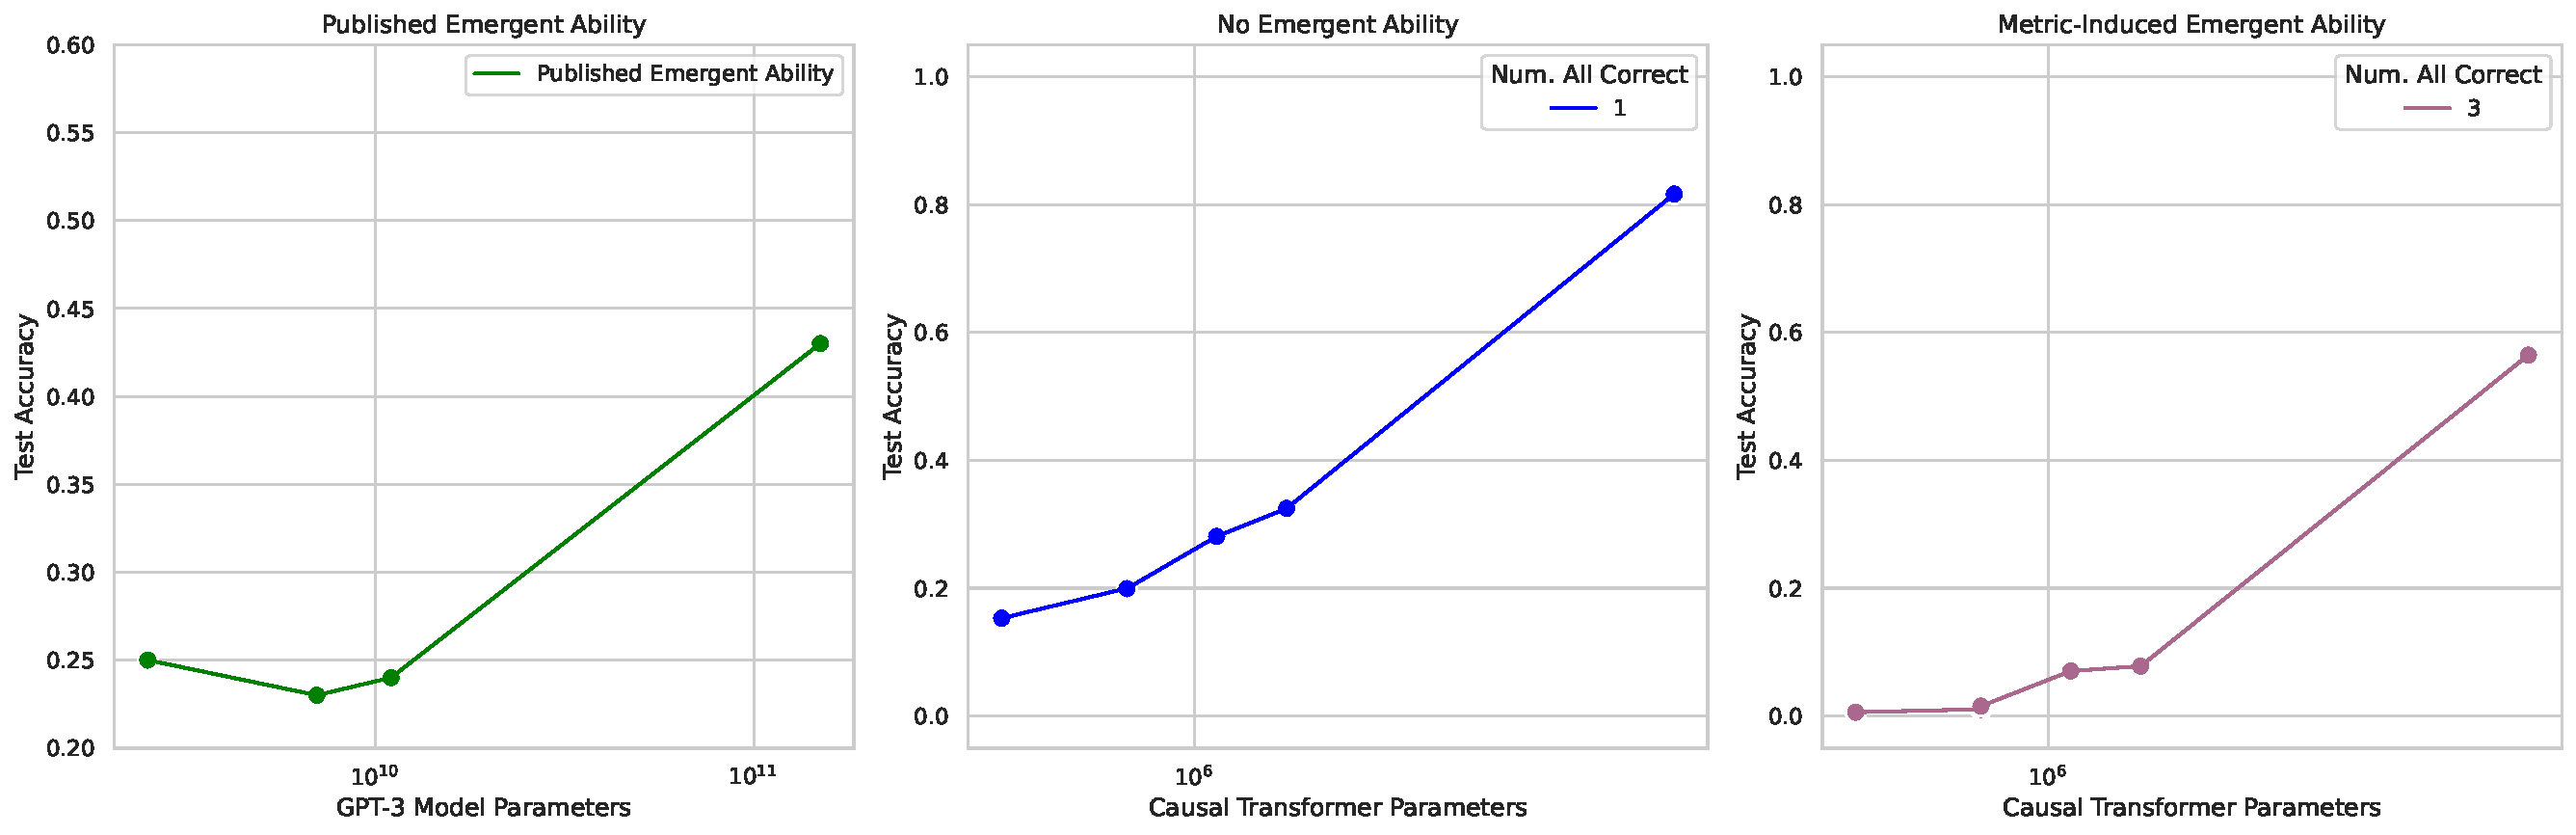
\includegraphics[width=0.9\textwidth]{figures/vision/no_emergence_and_emergence_dataset=omniglot.pdf}
    \caption{\textbf{Induced emergent classification ability in autoregressive Transformers.} (A) A published emergent ability on the MMLU benchmark \cite{ganguli2022predictability}. (B) Autoregressive transformers trained to classify Omniglot images display increasing accuracy with increasing scale. (C) When accuracy is redefined as classifying \textit{all} images correctly, a seemingly emergent ability appears.}
    \label{fig:vision_omniglot}
\end{figure}

We next induce emergent abilities in Transformers \cite{vaswani2017attention} trained to autoregressively classify Omniglot handwritten characters \cite{lake2015human}, in a setup inspired by recent work \cite{chan2022data}: Omniglot images are embedded by convolutional layers, then sequences of embedded image-image class label pairs are fed into decoder-only transformers.
We measure image classification performance on sequences of length $L \in [1, 5]$, again via \textit{subset accuracy}: $1$ if all $L$ images are classified correctly (Fig. \ref{fig:vision_omniglot}B), 0 otherwise.
Causal transformers display a seemingly emergent ability to correctly classify Omniglot handwritten characters (Fig. \ref{fig:vision_omniglot}C) that qualitatively matches published emergent abilities (Fig. \ref{fig:vision_omniglot}A).

% , e.g., Massive Multitask Language Understanding \cite{ganguli2022predictability}
